\chapter{Connectivity Hierarchy and Individual Contributions}
\label{contributions}

\section{Cooperation networks connectivity hierarchies as open elites}

The analysis of the hierarchical structure of organizations has been a central topic on organizational research in the last decades. This analysis has been mainly static in the sense that the focus of interest has been, among others, the distinctions between formal hierarchies and informal patterns of relations \citep{krackhardt:1993, mcfarland:2001}, the comparative analysis of the shape of the hierarchy \citep{blau:1962,blau:1964}, the impact of different kinds of hierarchical structures in the outcomes of the organizations' activities, the potential contradictions among the internal hierarchical structure of organization and its goals towards a more egalitarian society \citep{michels:1915,selznick:1949}, to cite only a few key issues.

Despite the huge among of work devoted to the analysis of hierarchy in organizations, the dynamic dimension of the hierarchy has received a lot less attention. The work on the dynamic dimension has focused on the evolution of hierarchical structures of organizations through time \citep{blau:1969}. There is however another possible definition of dynamic dimension in the analysis of hierarchy in organizations: the ratio of renewal of the individuals in the positions defined by that hierarchy. This important element of the dynamic dimension of hierarchy has been partially approached from the perspective of vacancy chains \citep{white:1970,stewman:1983}. However this approach has focused mostly on the career paths of individuals inside organizations instead of focusing on the pace of renewal of individuals in the hierarchical structure of organizations.

Our approach to analyze the structure and impact on individual contributions of connectivity hierarchies in cooperation networks follows the concept of open elite, first suggested by John Padgett in his statistical analysis of marriage patterns, family structure and elite reproduction in Florence between 1282 and 1494 \citep{padgett:2010}. In this work, Padgett suggests that despite a tendency to maintain an elite structure through marriages, the existence of three contending dimension of status (age of lineage, wealth and, political faction) led higher-status families to reach out and marry middle-tier ones, thus contributing unintentionally to social mobility. This approach leads to a ``reconceptualization of the concept of elite, more as a fluidly reproduced ideal than as a stable demographic reality'' \citep[360]{padgett:2010}. 

This reconceptualization was further developed in a study onf the emergence of commercial biotechnology in the United States, where \citet{powell:2005} identified an ``open elite'' network structure among dedicated biotech firms, pharmaceutical companies, venture capitalists, government agencies and universities which ``allowed for extensive crosstalk among a diverse set of organizations, melding practices and resources from multiple sources. Precisely because these organizations did not follow a common set of evaluative criteria, its heterogeneous, multiple affiliations made responsiveness to challenges possible.'' \citet[467]{powell:2005}.

We propose that hierarchical structures can be classified in a continuum, the two extreme points of which are, on the one hand, a static hierarchy ---where when an individual is appointed in a position of the hierarchy, this position is for life--- and, on the other hand, a dynamic hierarchy ---where the individuals occupying positions defined by the hierarchy have a very high pace of renewal. Notice that, in this context, the hierarchy can refer to both the formal and informal patterns of relations. An example of static hierarchy is the catholic church, where an appointment ---even far from the top level--- will typically last for life. On the other hand, dynamic hierarchies are a lot less common, especially before the last years of the twentieth century.

Since then we have witnessed the emergence of new organizational forms, mainly around Free and Open Source Software projects (FOSS). We propose that one of the central characteristics of these new organizational forms is precisely their high ratio of turnover in key hierarchical positions, both in the formal and informal internal organization. We do think that this dynamic dimension has not been taken into account in the analysis of those new organizational forms, and only by considering and analyzing it we can deepen our understanding, not only of the new emerging organizational forms, but also further our understanding of organizations and the challenges that they face.

In this chapter, we will start from this reconceptualization of an open elite in a dynamic hierarchy, and suggest that in FOSS projects there is a structural elite, identified as subgroups in the connectivity structure of their cooperation network that guarantee continuity and cohesion, but that these positions experience high membership turnover, and thus that this elite can be characterized as open.

\subsection{The dynamism of hierarchies in FOSS cooperation networks}

Free and Open Source Software (FOSS) communities have attracted a lot of attention from researchers of different fields since the late nineties of the past century. The first academic accounts of this phenomenon were mainly descriptive; their main focus was to just describe the organization of FOSS communities, the individual motivations of the people that form these communities, and the quality of the products that they produced \citep{benkler:2014}. Most of the interest was derived from the fact that FOSS communities do not conform to the accounts of collective dynamics and individual motivations established by the dominant neoclassical economic theories.

The academic efforts took mainly two directions. On the one hand, some authors tried to reconcile the dynamics of FOSS communities with neoclassical economic accounts. This effort was mainly focused on the individual motivations of the participants in those communities. They tried to explain these motivations in terms of rational self-interested individuals, as prescribed by dominant economic theories. On the other hand, other authors saw the emergence of FOSS communities as a new organizational form that provided a more democratic way of enabling collective production without the constrains imposed by the markets and/or bureaucratic organizational forms \citep{benkler:2002, benkler:2006, castells:2013}.

The later accounts of FOSS communities were initially uncritically celebratory of the phenomenon. They were heavily influenced by practitioners and advocates of the FOSS phenomenon which emphasized the technical superiority of the products developed by FOSS communities, while maintaining an ethical stand that valued more cooperation and reciprocity than competition and self-interest. One of the most influent early accounts from practitioners was \citet{raymond:1999} that proposed, among other things, that the technical superiority of FOSS software products was due to the ``Linus law'', which states that ``given enough eyeballs, all bugs are shallow'', suggesting that given a large enough developer and user community with access to the source code, all software errors (ie ``bugs'') will be detected quickly and the solution will be obvious at least to someone.

Thus ``Linus law'' suggests that FOSS communities are composed by a large set of individuals loosely organized with a very flat or inexistent hierarchy among them, and that all individuals might contribute more or less the same: a pair of eyes that should look at the source code in order to improve it. This somewhat naive account of the dynamics of FOSS production process was accepted uncritically by many academics that were sympathetic with the arguments of the FOSS practitioners. Some critical voices, coming mostly from Computer Science, challenged this claim with sound empirical arguments; for instance \citet{glass:2002} correctly noted that if ``Linus Law'' was right then the number of bugs found in a software project should increase linearly with the number of people looking at their source code. No such thing have been proved empirically. Also, ``Linus Law'' not only treats each pair of eyes (ie individuals) as equally important, it also implicitly assumes that all bugs are similar, which is very implausible.

Other early empirical research, coming mostly from Computer Science, has pointed out that even in big, mature and widely used FOSS projects, only few of the participants account for the lion's share of the work done. For instance, \citet{mockus:2002} show that less that 20 developers of the Apache project\footnote{Apache is one of the most successful FOSS projects, it's flagship product is the Apache web server which powers more than 50\% of the web sites that form the WWW.} contributed more than 80\% of the code base. This core of developers is embedded in a larger set of participants, that mainly help reporting and fixing errors, answering questions about the software in public forums, and writing documentation. Later empirical research has confirmed that the distribution of contributions in FOSS projects is right-skewed and heavy tailed, meaning that most participants make very small contributions, and only few individuals make almost all relevant contributions.

Recent empirical research on peer production projects (concretelly user edited wikis) has also shown that these projects exhibit deep contribution inequalities \citep{shaw:2014}. The authors suggest that these projects may conform to \citet{michels:1915} ``iron law of oligarchy'' which states that organizations tend towards oligarchy as they grow, even if democracy and participation are part of the core goals of the organization. Therefore, there is ample empirical evidence that confirms that there is an important differentiation of roles and functions among participants on FOSS communities. This fact does not fit well with the picture of a flat hierarchy of peers portrayed by early accounts of the phenomenon.

We do think that the narrative of a flat hierarchy of peers was so successful because the formal organization of most FOSS projects is usually quite fuzzy, and very different of the formal structure of other kinds of organizations. However, the informal structure emerging from the patterns of cooperation among individuals in a FOSS project is quite hierarchical because reflects the fact that only few individuals are responsible for most contributions to the project. We propose that the way to advance our theoretical understanding of the FOSS phenomenon is by analyzing their social structure. The social structure of a community are the patterns of relations established among individual participants in the process of building the software packages (or any other product, such as on on-line encyclopedia) that they release. The public nature of FOSS communities implies that most of the data generated in the production process is available, and thus an important source of empirical data that we can use to test competing theoretical accounts of the phenomenon. 

We found that the developers that contribute the most are in the higher levels of the connectivity structure of the project's cooperation networks. Moreover, by analyzing the composition of individuals on these key topological positions we are able to assess to which extend there is turn over of individuals at the top of the connectivity structure. Our analysis shows that the ratio of renewal of individuals at this structural position is quite fast, which characterizes FOSS communities as dynamic hierarchies. Thus, if we analyze cross-sectionally (ie in a concrete point of time) a FOSS project, a very small fraction of the participants are the ones that actually do the lion's share of contributions, as previous empirical research has shown. However if we analyze the evolution of contributions longitudinally, we find that the persons that contribute the most change through time. This continuous renewal of the people that does most of the work ---what we call dynamic hierarchy--- is a key mechanism to explain how FOSS projects, which are mostly voluntary based, geographically distributed, and mostly operated from the Internet, can thrive and evolve to a point where they are key pieces of the infrastructure that enables the Internet and other essential Information technologies.

Our focus on the rotation of individuals at the top levels of the connectivity structure brings us to the issue of the robustness of the FOSS communities. From a pure network perspective, it is usual to analyze robustness by removing nodes and measuring how this affects the size of the giant connected component in the network \citep{albert:2000}. Nodes are removed following different mechanisms; either at random ---to simulate failure--- or removing nodes according to their degree ---to simulate a deliberate attack. However these mechanisms are best suited for analyzing the robustness of physical networks, such as the Internet. They clearly fall short for analyzing the robustness of FOSS communities, because not random failures nor targeted attacks are the main mechanisms through which the persons that work on FOSS communities turn over.

Our approach here is to analyze the median active life of developers in a FOSS project as a better way of assessing the robustness of a FOSS community. We also apply the well established survival analysis techniques \citep{miller:2011} in order to describe and model the flux of people throughout the history of a FOSS community.  We found that the position of an individual in the connectivity structure of the collaboration network also impacts significantly in the median life of a developer in the project.

\section{Methods}

In this chapter we analyze the role of the connectivity structure of the cooperation networks in shaping individual contributions to Debian and Python projects. We focus on the structural positions in which the most active contributors are, and the median life of individual contributions on the project. Our main empirical interest is about the volume of contribution of each individual to the project, and the role of contributions ---as independent variable--- in relevant elements of a FOSS project, such as the median active life of individual contributors to the project.

Our modeling strategy to capture the patterns of relations among developers in these two projects is to focus on the actual contributions of each developer to the project. Following our approach in the previous chapter, we model cooperation networks as bipartite graphs, where the two sets of nodes are, on the one hand, human developers and, on the other hand, entities that conform the product that is released by the FOSS project. In the case of Debian, these entities are software packages, and in the case of Python, they are source code files. Note that the collaboration network is based on individual contribution but it not only captures the total amount of contribution that a given individual does, but also to which part of the project the contributions are focused, and who else in the project is also working on the same entities. This is why we name these bipartite graphs cooperation networks.

This modeling approach captures mostly the informal patterns of relations that individuals establish when contributing to the project. FOSS projects have a wide range of formal organizational forms, and in this respect, they can be quite different. The definition of the leadership position in the two projects in which we focus this paper nicely capture these differences in formal organization: Debian has a very developed formal bureaucracy, the project elects its leader each year through a secret vote of all its members after a electoral campaign where the candidates discuss among them and try to gain supports; Python instead has its original author ---Guido van Rossum--- in a permanent position of leadership, the people in the project refer to him, and his position of leadership, as ``Benevolent Dictator For Life'' (BDFL).

Despite these differences in the formal organization, if we focus on the patterns of relations among developers in the productive process, what we call the collaboration network, we can analyze the contribution dynamics, analyze hierarchical positions defined by these patterns, assess the pace of renewal in these positions, and determine the impact in the median active life on a developer in a project of being in a concrete hierarchical position.

One of the challenges that we faced, that is both theoretical and methodological, is how to define cohesive groups in collaboration networks. There are many ways of defining a cohesive group given a collaboration network. Our aim was to define groups in cooperation networks in a way that is theoretically sound from a sociological point of view. Network science is nowadays quite interdisciplinary, and a lot of physicist have recently proposed a bunch of techniques, under the label of community detection algorithms \citep{fortunato:2010}, that determine groups in networks based on the patterns of relations among the entities of the network.

However, these techniques are suboptimal from a sociological theory point of view because the four key elements that a sociologically sound group classification should have are not present in most, if not all, most used community detection algorithms, as discussed in chapter \ref{structural_cohesion} (and published at \citep{torrents:2015}). The four key dimensions are: robustness (the groups should not depend on only one or few individuals to be a group), overlap (persons usually are part of more than one cohesive group), positional dimension (some actors, because of their position in the global patterns of relations, obtain preferential access to information or resources that flow through the network), and hierarchy (cooperation networks have \emph{hierarchical structure} in the sense that highly cohesive subgroups are nested inside less cohesive ones).

Our conclusion is that the structural cohesion model, developed by White, Moody and Harary \citep{white:2001, moody:2003}, is the best model for analyzing group formation in cooperation networks in the context of our empirical research. This model is based on the graph theoretic measure of node connectivity, and defines cohesive groups as $k$-components, that is, groups of nodes in which $k$ nodes have to be removed in oder to disconnect the group. $K$-components form the connectivity structure of the network, and aptly capture the central elements of a sociological definition of cohesive group \citep{torrents:2015}.

However, there are some important practical difficulties related to the computation of the measures that characterize the structural cohesion model. Their time complexity is super quadratic, approximately of the order of the forth power of the size of the input network. This makes non practical the exact computation of the k-component structure in networks bigger than several hundreds of nodes. We use here some useful heuristics that allow to approximately compute the connectivity structure of large sparse networks in a reasonable time frame, as we have shown in chapter \ref{structural_cohesion}.

Once we built the cooperation networks for the two projects, and determined their connectivity structure, we perform a descriptive analysis of the percentage of total contributions by connectivity level. This simple descriptive analysis shows that there is a strong correlation between the position of a developer in the connectivity structure of the cooperation network and her total amount of contribution to the project.

We then deepen our analysis by modeling individual contributions to the project using different regression models in order to asses the relation of the structural positions that individuals occupy with their level of contribution to the project. For the case of the Debian project, contributions are uploads of packages to the central repository of the project, thus contributions in this context have to be modeled as a discrete variable. For this case we used a negative binomial regression model to deal with the over-dispersed count data from the values of the discrete contributions variable.

For the case of the Python project, contributions are lines of source code added or deleted from one of the source code files of Python's code base. We modeled contributions using a panel regression with individual fixed effects. This design allows us to account for unobserved variability among the individual developers, such as cultural background or coding expertise, and disentangle if the position of a developer in the connectivity hierarchy has an effect in her level of contribution to the project.

Finally, we are also interested in the impact of the position than an individual occupies in the cooperation network with her long term involvement with the project. To that end we applied Cox proportional-hazards regression for survival data to both Debian and Python projects. In its origin, survival analysis, was focused on modeling lifespans of individuals and is still widely used in medicine. However, this kind of analysis can also be used to model any kind of duration. We model the active life of a developer in a FOSS project to the period that this developer doing at least one contribution. We consider a developer ``dead'' when she no longer contributes.

\section{Results}

\subsection{Modeling individual contributions}

As we discussed, the empirical work on FOSS communities has already established that it is only a small fraction of all participants in a project who are responsible for most contributions. As a first step for our analysis, we analyze the topological position of the individuals that contribute the most in the patterns of relations ---the social structure--- among individuals in that project. Following our proposed cohesive small world model (see chapter \ref{collaborative_communities}), and one of its foundaments: the structural cohesion model \citep{moody:2003} (see chapter \ref{structural_cohesion}), we found that these individuals are part of the top connectivity levels of the cooperation network, that is, they are members of $k$-components of high $k$ which represent cohesive subgroups nested inside each other in the network that emerges from the patterns of relation among developers in the productive process. 

\begin{figure}[h]
%\centering
\subfloat[Evolution of the percentage of developers by connectivity level for the Debian project.]{
\label{fig:evo-sc}
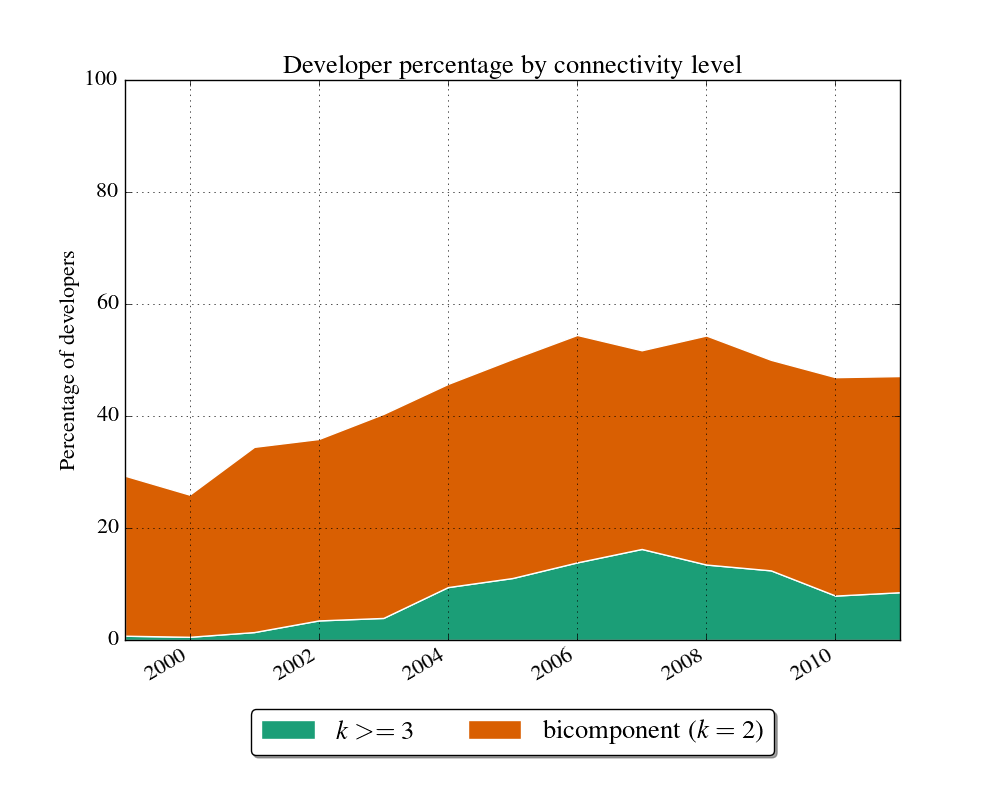
\includegraphics[scale=0.29]{figures/evolution_developers_debian_years}
}
\hspace{.05in}
\subfloat[Evolution of the percentage of contributions by developers by connectivity levels for the Debian project.]{
\label{fig:evo-contrib}
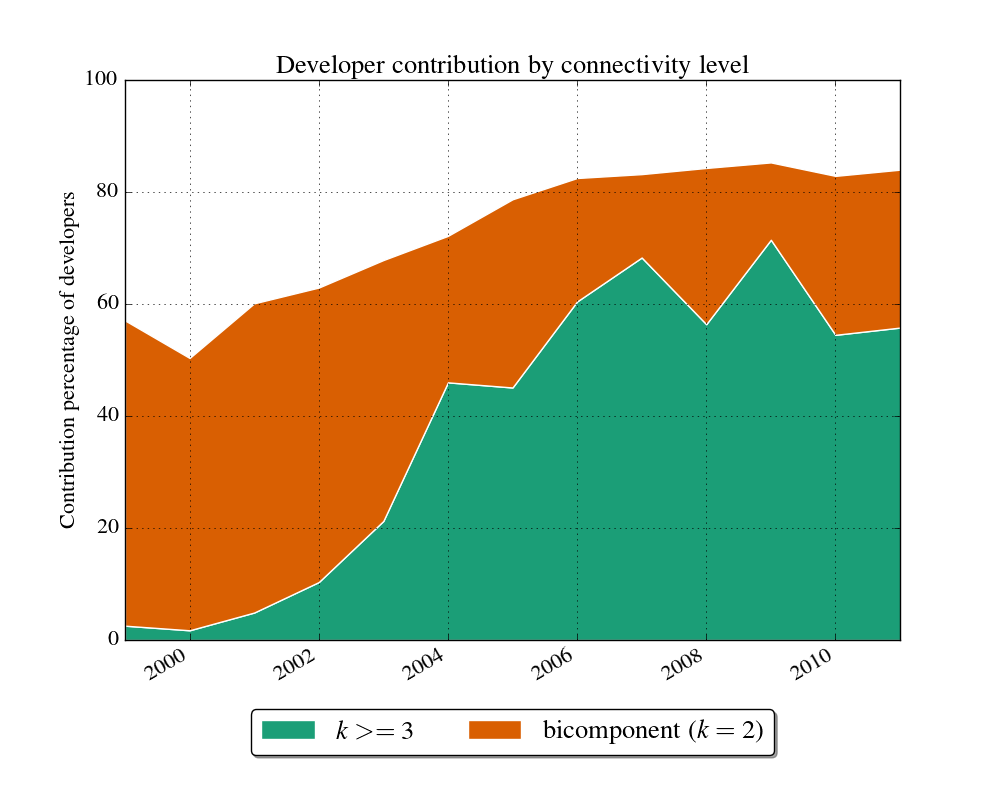
\includegraphics[scale=0.29]{figures/evolution_connectivity_debian_years}
}

\caption[Debian: Evolution of connectivity levels and contributions.]{Evolution of the percentage of developers in each connectivity level (left) and evolution of the percentage of contributions by developers by connectivity levels (right) for the Debian project. The green surface represents the developers in the top connectivity levels, that is developers that are part of a $k$-component with $k$ greater or equal than 3. The orange surface represents developers in bicomponents, that is $k$-components with $k=2$.}
\label{fig:evo}
\end{figure}

Figure \ref{fig:evo-sc} displays the evolution of the percentage of developers by connectivity level in the period under analysis. The green surface represents the developers in the top connectivity levels, that is developers that are part of a $k$-component with $k$ greater or equal than 3. The orange surface represents developers in bicomponents, that is $k$-components with $k=2$. Note that all developers in the top connectivity levels are also part of the bicomponents. In the period under analysis, there is a significant increment of the hierarchy of connectivity levels, as we have shown in the previous chapter, which peaks in 2007 with 17\% of the developers in connectivity levels with $k \ge 3$. The percentage of developers in bicomponents, goes from 26\% in 2002 to 50\% in 2005 and peaks at almost 54\% of developers at 2006 and 2008. From 2005 to the end of the period under analysis the percentage stabilizes between 45\% and 54\%. The percentage of developers in higher connectivity levels also experiments an important increment, it goes from less than 1\% in 1999 and 2000 to 8\% in 2011, and peaks around 16\% in 2007.

Figure \ref{fig:evo-contrib} displays the percentage of contributions by developers by connectivity level. We can see that, although there are few developers in high connectivity levels, they are responsible for a big fraction of the total contribution in terms of packages uploaded to the Debian archive. For instance, in 2004 the develoeprs in the top connectivity levels were less tha 10\% of all developers, but they contributed 46\% of all uploads to the Debian repository that year. That same year, 45\% of the developers were embbeded in a bicomponent and contributed 72\% of all uploads. In 2009, 12.5\% of the developers that were part of the top connectivity levels were responsible for 71\% of all contributions, while developers in $k$-components with $k \ge 2$ contributed 85\% of all uploads while being only 50\% fo all developers that uploaded at least one package to the Debian archive that year. 

Therefore, it is clear that there is a strong correlation between the connectivity level of a developer and her contribution to the project. To further the analysis, we modeled the contributions ---which in this case are uploads of new versions of packages to the Debian archive--- using a negative binomial regression. Which is well suited for the count nature of our dependent variable (\# of uploads) and its over dispersion. We cannot use a zero inflated model in this case because by design there is no zeros in the dataset as we only considered developers that have at least uploaded one package. This regression model is not for all the period analyzed on our previous analysis (1999-2012) because the scale of the Debian system ---in terms of the number of packages--- has grown too much in this period and thus the later years would have been overrepresented. We opted for analyzing the developement time of a complete version of the Debian syste. Concretelly we analyzed the period from 2011-02-06 to 2013-05-04  corresponding to the developement cycle of the Debian release 7.0 codename Wheezy.

We controlled the contributions of each developer, on the one hand, by several key variables related to the technical side of the production process, such as the size (\emph{log(Package size)}) and the dependencies of each package (\emph{\# of package dependencies}), the bugs reported for each package (\emph{\# of bugs reported}), or the time that the developer has been active in the project (\emph{Developer tenure (years)}). And, on the other hand, we also controlled for centrality measures including degree centrality (\emph{Degree centrality}) and closeness (\emph{Closeness}), and a local cohesion metric (\emph{Square Clustering}). As can be seen in table \ref{debian_nbinomial}, the connectivity level in which a developer is embedded (\emph{$k$-component number}) has a positive and significative impact on her contributions to the project.


% Table created by stargazer v.5.2 by Marek Hlavac, Harvard University. E-mail: hlavac at fas.harvard.edu
% Date and time: dj, nov 17, 2016 - 04:01:12
% Requires LaTeX packages: dcolumn 
\begin{table}[!htbp] \centering 
  \caption{Negative binomial model for Debian uploads} 
  \label{debian_nbinomial} 
\begin{tabular}{@{\extracolsep{5pt}}lD{.}{.}{-3} D{.}{.}{-3} D{.}{.}{-3} D{.}{.}{-3} } 
\\[-1.8ex]\hline 
\hline \\[-1.8ex] 
 & \multicolumn{4}{c}{\textit{Dependent variable:}} \\ 
\cline{2-5} 
\\[-1.8ex] & \multicolumn{4}{c}{Number of uploads by developer} \\ 
\\[-1.8ex] & \multicolumn{1}{c}{(1)} & \multicolumn{1}{c}{(2)} & \multicolumn{1}{c}{(3)} & \multicolumn{1}{c}{(4)}\\ 
\hline \\[-1.8ex] 
 Intercept & -0.647^{*} & -0.545^{**} & -0.837^{***} & -1.453^{***} \\ 
  & (0.262) & (0.199) & (0.200) & (0.191) \\ 
  log(Package size) & 0.309^{***} & 0.229^{***} & 0.240^{***} & 0.203^{***} \\ 
  & (0.021) & (0.016) & (0.016) & (0.015) \\ 
  \# of bugs reported & -0.007^{***} & 0.002 & 0.002 & 0.001 \\ 
  & (0.002) & (0.001) & (0.001) & (0.001) \\ 
  \# of package dependencies & -0.020^{**} & -0.016^{**} & -0.017^{**} & -0.021^{***} \\ 
  & (0.008) & (0.006) & (0.006) & (0.005) \\ 
  Developer tenure (years) & 0.105^{***} & 0.071^{***} & 0.077^{***} & 0.083^{***} \\ 
  & (0.008) & (0.006) & (0.006) & (0.006) \\ 
  Degree centrality &  & 47.333^{***} & 47.318^{***} & 27.174^{***} \\ 
  &  & (0.695) & (0.691) & (0.742) \\ 
  Closeness &  & -0.304 & -0.142 & 0.651^{***} \\ 
  &  & (0.179) & (0.180) & (0.175) \\ 
  Square clustering &  &  & 0.421^{***} & 0.055 \\ 
  &  &  & (0.077) & (0.077) \\ 
  k-component number &  &  &  & 0.690^{***} \\ 
  &  &  &  & (0.032) \\ 
 \hline \\[-1.8ex] 
Observations & \multicolumn{1}{c}{1,750} & \multicolumn{1}{c}{1,750} & \multicolumn{1}{c}{1,750} & \multicolumn{1}{c}{1,750} \\ 
Log Likelihood & \multicolumn{1}{c}{-8,235.163} & \multicolumn{1}{c}{-7,541.388} & \multicolumn{1}{c}{-7,528.735} & \multicolumn{1}{c}{-7,393.372} \\ 
Akaike Inf. Crit. & \multicolumn{1}{c}{16,480.330} & \multicolumn{1}{c}{15,096.770} & \multicolumn{1}{c}{15,073.470} & \multicolumn{1}{c}{14,804.740} \\ 
\hline 
\hline \\[-1.8ex] 
\textit{Note:}  & \multicolumn{4}{r}{$^{*}$p$<$0.05; $^{**}$p$<$0.01; $^{***}$p$<$0.001} \\ 
\end{tabular} 
\end{table} 


Tables \ref{desc_table_nbinomial} and \ref{corr_table_nbinomial} on appendix \ref{support-tables} show the descriptive statistics and the correlation matrix of the variables used in this model. In terms of the importance of the variables in the model, our independent variable $k$-number (the value $k$ of the connectivity level in which the developer is embedded in the connectivity hierarchy) is the second most important only after degree centrality. We measure variable importance here as normalized magnitude by dividing the coefficient in the model by its standard deviation.
 
The fact that the quantification of contributions in the Debian project is a discrete variable ---number of package uploads to the Debian repository--- restricts the options of regression modeling available. The over dispersed negative binomial regression is clear in that the connectivity level in the collaboration network has a positive and significant impact on the level of contribution of each developer. However it does not allow to take into account unobserved individual differences among developers that might explain their level of contribution.

Another source of concern with this model it's the potential endogenity of the relation between the dependent variable and the network metrics, which include our independent variable. Given that the cooperation network is build preciselly based on uploads to the Debian archive, which is the dependent variable in this model. We will refine our analysis to deal with endogenity problems using data from the Python project. 

As discussed above, the data from Python project allows us to measure contributions as lines of source code added by each developer. This variable can be safely considered continuous and therefore we can model it as a panel regression with individual and time fixed effects. This modeling approach, on one hand, solves the problem of unobserved differences between developers that might have an effect of the volume of their contributions, and on the other hand, also allows to account for changes in system through time that we were not able to model in the negative binomial regression of table \ref{debian_nbinomial}.
 
Let's first take a look at the descriptive data on percentage of contributions by the top connectivity level (the developers that are in the $k$-component with the highest $k$) in the Python project. Figure \ref{fig:composition} displays the evolution of percentage of developers that are at the top connectivity level throughout the history of Python project. The orange surface shows the percentage of developers that are included in the giant bicomponent, and the green surface represents the percentage of developers in the top connectivity level, that is the $k$-component of maximum $k$ in the cooperation network of that year.

We can see that around 40\% of the developers that have contributed some code are in the top level of the connectivity hierarchy, and this percentage is quite stable through time. Note that the actual $k$ value of the top level varies in time, depending on how the patterns of relations among developers and source code files have evolved each concrete year. The node connectivity of the $k$-component in the top of the connectivity hierarchy is almost all years between 7 and 10, with a minimum of 6 in 2005.

\begin{figure}[h]
\centering
\subfloat[Evolution of the percentage of developers by connectivity level for the Python project.]{
\label{fig:composition}
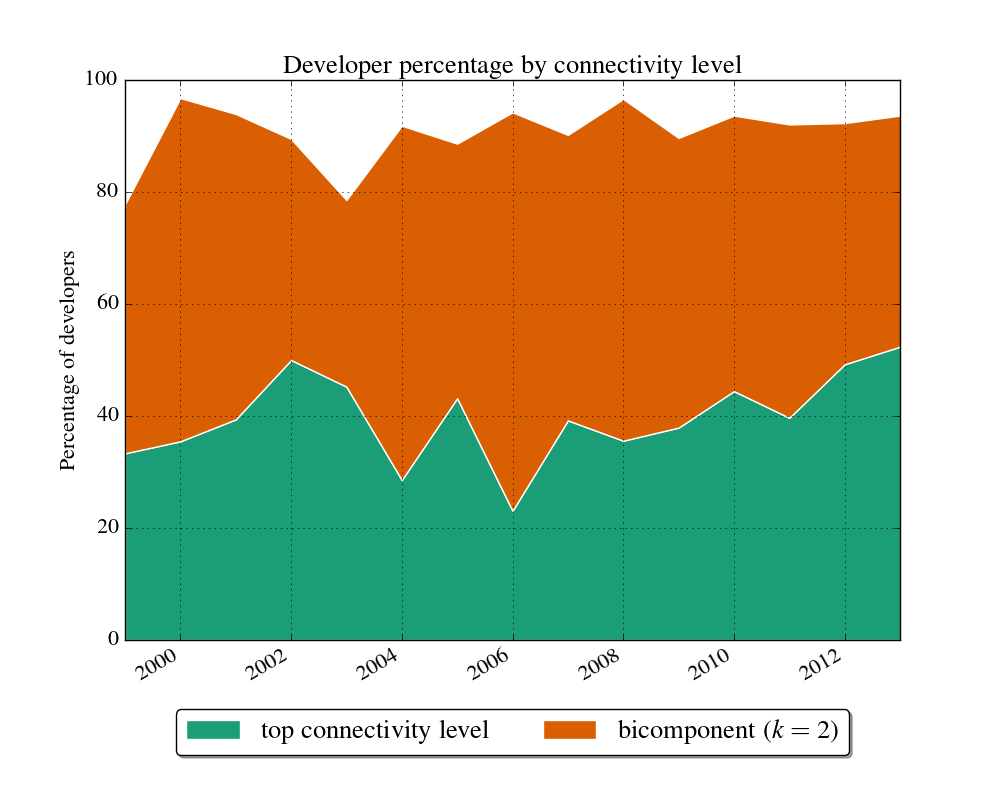
\includegraphics[scale=0.29]{figures/evolution_developers_python_years}
}
\hspace{.01in}
\subfloat[Evolution of the percentage of contributions by developers by connectivity levels for the Python project.]{
\label{fig:contributions}
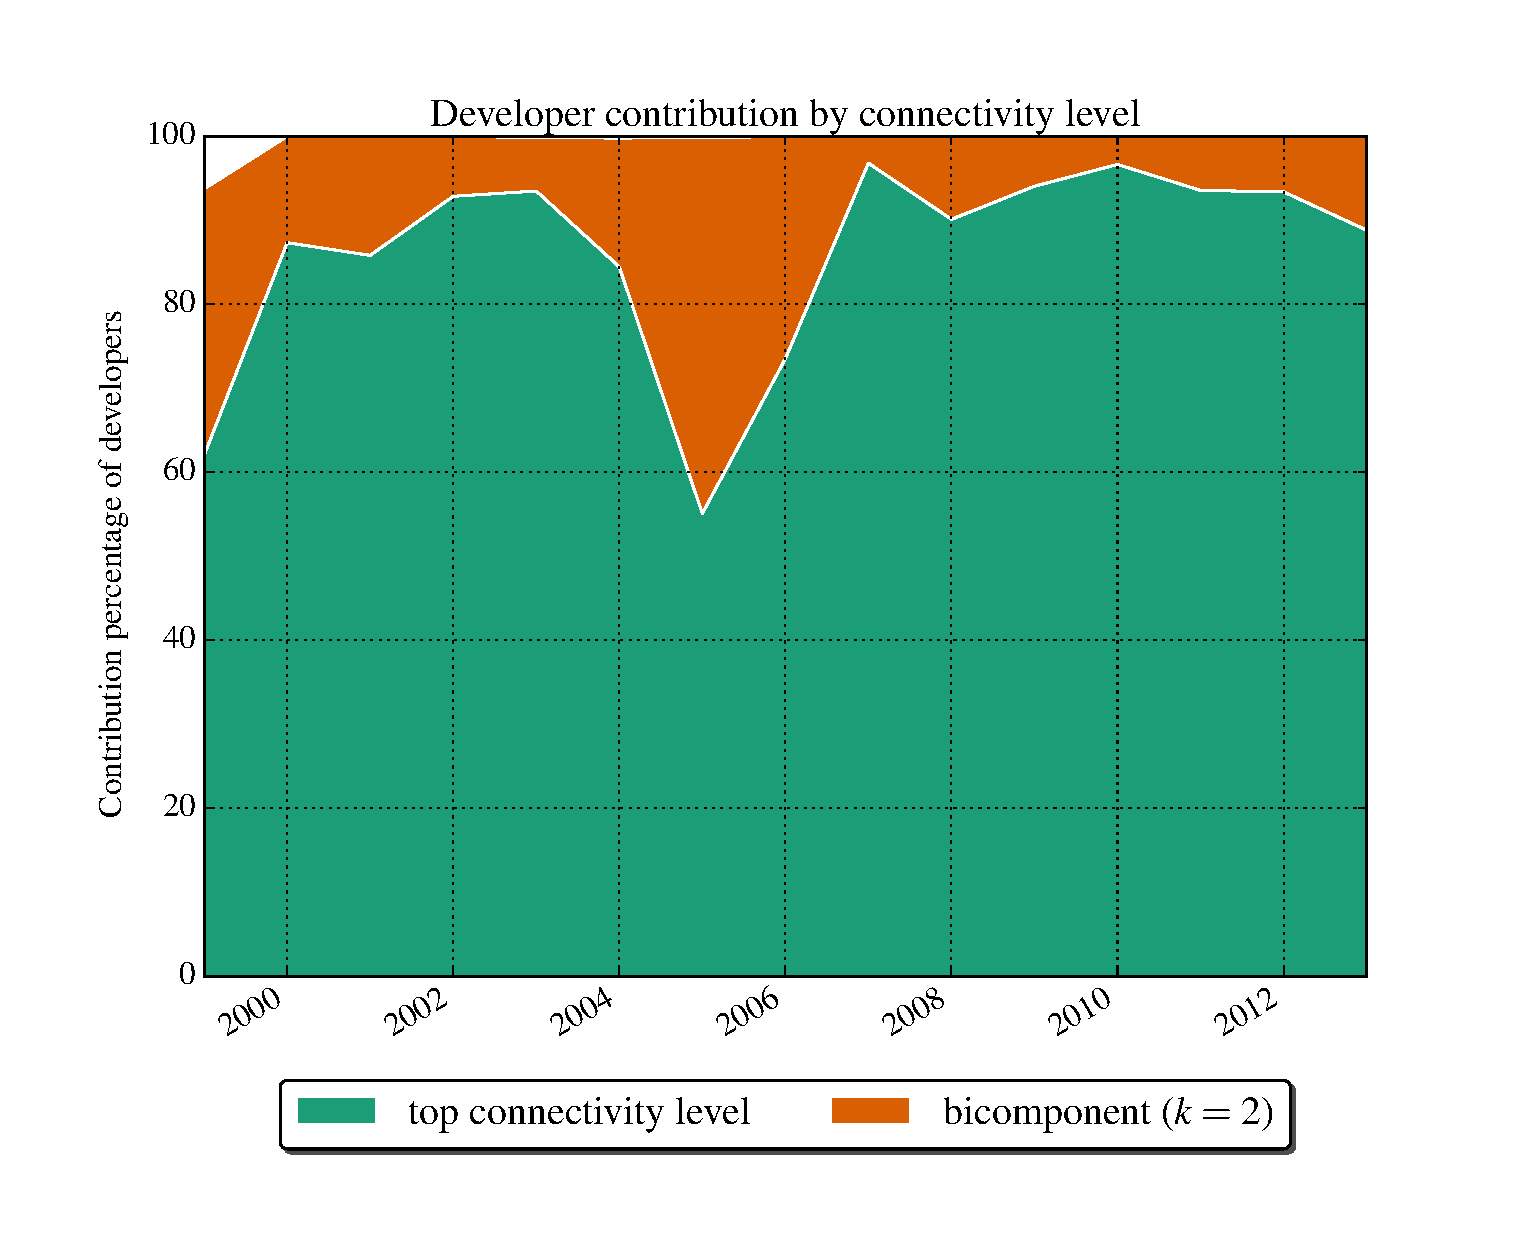
\includegraphics[scale=0.29]{figures/evolution_connectivity_python_years}
}
\label{fig:comp_and_contrib}
\caption[Python: Evolution of connectivity levels and contributions.]{Evolution of the percentage of developers by connectivity level (left) and evolution of the percentage of contributions by developers by connectivity levels (right) in the Python project. The green surface represents the developers in the top connectivity level, that is developers that are part of a $k$-component with maximum $k$. The orange surface represents developers in bicomponents, that is $k$-components with $k=2$.}
\end{figure}

Figure \ref{fig:contributions} shows the evolution of the contributions of the developers by connectivity level, measured in terms of lines of source code added to the project. Note that $k$-components are nested inside each other, like Russian dolls, thus the contributions of developers in the giant biconnected components also include the contributions of the developers in the top connectivity level. As we can see, developers in the giant biconnected component are the authors of almost all contributions, but they are also between 80\% and 97\% of all developers.

However developers in the top connectivity level are only between 40\% and 55\% of all developers on the project, but they are the authors, the latter years of the period under analysis, of around 90\% of the source code contributions. Some years their percentage of contributions is lower (a bit less than 60\%) but this is mostly before 2001, when the community was much smaller than in the following years, or in 2005. Therefore only a small fraction of the developers are responsible of the lion's share of the work done in the project. Note however that the contributions to source code files, what is measured here as contributions, does not include all the work done that is important to the project, such as managing the infrastructure for distributing Python, helping users in the mailing list, maintaining the websites of the project, etc ... 

For modeling individual contributions to the Python project, we used a panel regression with individual and year fixed effects. This design allows us to account for unobserved variability among the individual developers, such as cultural background or coding expertise, and disentangle if the position of a developer in the connectivity hierarchy has an effect in her level of contribution to the project. As we can see in the table, being in the top connectivity level has a positive and significant impact in the level of contribution of each developer. Note also that considering the $k$-number of the developer (ie, the level $k$ of the highest $k$-component in which the developer is embedded) adds explanation power on the model and suggest that the impact of the connectivity hierarchy on the productivity of developers operates at all connectivity levels, not only at the top.

The model also includes control variables for the centrality of each developer in the collaboration network (Degree centrality and Closeness), the number of direct collaborators of each developer (collaborators), the tenure of each developer (measured as the number of years since their first contribution) and the value of square clustering which is a measure of local cohesion. Tables \ref{desc_table_panel} and \ref{corr_table_panel} on appendix \ref{support-tables} show the descriptive statistics and the correlation matrix of the variables used in this model.


% Table created by stargazer v.5.2 by Marek Hlavac, Harvard University. E-mail: hlavac at fas.harvard.edu
% Date and time: dj, nov 17, 2016 - 03:57:39
% Requires LaTeX packages: dcolumn 
\begin{table}[!htbp] \centering 
  \caption{Contributions Fixed Effects Panel Regression Results} 
  \label{} 
\begin{tabular}{@{\extracolsep{5pt}}lD{.}{.}{-3} D{.}{.}{-3} D{.}{.}{-3} D{.}{.}{-3} } 
\\[-1.8ex]\hline 
\hline \\[-1.8ex] 
 & \multicolumn{4}{c}{\textit{Dependent variable:}} \\ 
\cline{2-5} 
\\[-1.8ex] & \multicolumn{4}{c}{Lines of Source Code} \\ 
\\[-1.8ex] & \multicolumn{1}{c}{(1)} & \multicolumn{1}{c}{(2)} & \multicolumn{1}{c}{(3)} & \multicolumn{1}{c}{(4)}\\ 
\hline \\[-1.8ex] 
 Degree Centrality & 7.053^{***} & 7.040^{***} & 5.779^{***} & 5.997^{***} \\ 
  & (0.887) & (0.891) & (0.797) & (0.642) \\ 
  Collaborators & 0.086^{***} & 0.086^{***} & 0.072^{***} & 0.038^{***} \\ 
  & (0.006) & (0.006) & (0.006) & (0.006) \\ 
  Tenure (years) & -0.260^{***} & -0.262^{***} & -0.199^{***} & -0.131^{***} \\ 
  & (0.030) & (0.030) & (0.029) & (0.032) \\ 
  Closeness & -0.709 & -0.725 & 0.140 & -0.465 \\ 
  & (0.809) & (0.815) & (0.828) & (0.973) \\ 
  Square clustering &  & -0.092 & 0.211 & 0.580 \\ 
  &  & (0.364) & (0.336) & (0.299) \\ 
  Top connectivity level &  &  & 1.202^{***} & 0.579^{**} \\ 
  &  &  & (0.186) & (0.177) \\ 
  k-component number &  &  &  & 0.330^{***} \\ 
  &  &  &  & (0.047) \\ 
 \hline \\[-1.8ex] 
Observations & \multicolumn{1}{c}{816} & \multicolumn{1}{c}{816} & \multicolumn{1}{c}{816} & \multicolumn{1}{c}{816} \\ 
Adjusted R$^{2}$ & \multicolumn{1}{c}{0.388} & \multicolumn{1}{c}{0.387} & \multicolumn{1}{c}{0.420} & \multicolumn{1}{c}{0.464} \\ 
\hline 
\hline \\[-1.8ex] 
\textit{Note:}  & \multicolumn{4}{r}{$^{*}$p$<$0.05; $^{**}$p$<$0.01; $^{***}$p$<$0.001} \\ 
\end{tabular} 
\end{table} 


This regression modeling of Python contributions by connectivity level complements and confirms the negative binomial regression results applied to the Debian project. The $k$-components of the cooperation network define groups of developers that are the core of the project and are responsible for most of the contributions, both in Debian and in Python project. These groups are central in a structural sense as they are at the top of the connectivity hierarchy that emerges from the patterns of cooperation among individual developers. The models presented thus far point out that these developers are also the ones responsible for the lion's share of the contributions, and thus the hierarchical structure of the coopreration network shapes the volume of contribution of individual developers.

However the fixed effects panel regression also has a potential problem of endogenity as the cooperation network form which we computed the connectivity hierarchy is based on individual contributions and this was our dependent variable in both this regression model and the negative binomial model we explored before for the case of the Debian project. Note that despite this potential problem, if we look at the correlation tables for these models at appendix \ref{support-tables}, we can see that the correlations between the independent and dependent variables is not high enough ---0.488 for the negative binomial and 0.211 for the fixed effects panel regression--- to create coliniality problems in the models.


% Table created by stargazer v.5.2 by Marek Hlavac, Harvard University. E-mail: hlavac at fas.harvard.edu
% Date and time: dj, nov 17, 2016 - 03:57:56
% Requires LaTeX packages: dcolumn 
\begin{table}[!htbp] \centering 
  \caption{Zero Inflated negative binomial model for PEPs} 
  \label{python_zinfl} 
\begin{tabular}{@{\extracolsep{5pt}}lD{.}{.}{-3} D{.}{.}{-3} D{.}{.}{-3} D{.}{.}{-3} } 
\\[-1.8ex]\hline 
\hline \\[-1.8ex] 
 & \multicolumn{4}{c}{\textit{Dependent variable:}} \\ 
\cline{2-5} 
\\[-1.8ex] & \multicolumn{4}{c}{Total number of accepted PEPs authored} \\ 
\\[-1.8ex] & \multicolumn{1}{c}{(1)} & \multicolumn{1}{c}{(2)} & \multicolumn{1}{c}{(3)} & \multicolumn{1}{c}{(4)}\\ 
\hline \\[-1.8ex] 
 log(\# of lines of code authored) & 0.070 & 0.011 & 0.026 & 0.009 \\ 
  & (0.037) & (0.038) & (0.043) & (0.042) \\ 
  Degree Centrality & 1.507^{*} & 1.135 & 1.655^{*} & 1.151 \\ 
  & (0.728) & (0.662) & (0.724) & (0.673) \\ 
  Tenure (years) & 0.177^{***} & 0.180^{***} & 0.176^{***} & 0.180^{***} \\ 
  & (0.012) & (0.011) & (0.012) & (0.011) \\ 
  Collaborators & 0.018^{*} & 0.011 & 0.011 & 0.011 \\ 
  & (0.008) & (0.007) & (0.008) & (0.008) \\ 
  Closeness & -5.688^{*} & -4.661^{*} & -5.433^{*} & -4.659^{*} \\ 
  & (2.574) & (2.240) & (2.540) & (2.240) \\ 
  Square clustering & -0.416 & -0.108 & -0.239 & -0.103 \\ 
  & (0.266) & (0.268) & (0.278) & (0.274) \\ 
  Top connectivity level &  & 0.683^{***} &  & 0.675^{***} \\ 
  &  & (0.163) &  & (0.181) \\ 
  k-component number &  &  & 0.093^{*} & 0.006 \\ 
  &  &  & (0.047) & (0.051) \\ 
  Constant & 0.878 & 0.589 & 0.611 & 0.579 \\ 
  & (0.921) & (0.835) & (0.921) & (0.842) \\ 
 \hline \\[-1.8ex] 
Year dummies:  & \multicolumn{1}{c}{Yes} & \multicolumn{1}{c}{Yes} & \multicolumn{1}{c}{Yes} & \multicolumn{1}{c}{Yes} \\ 
\hline \\[-1.8ex] 
Observations & \multicolumn{1}{c}{773} & \multicolumn{1}{c}{773} & \multicolumn{1}{c}{773} & \multicolumn{1}{c}{773} \\ 
Log Likelihood & \multicolumn{1}{c}{-1,083.697} & \multicolumn{1}{c}{-1,073.610} & \multicolumn{1}{c}{-1,081.423} & \multicolumn{1}{c}{-1,073.576} \\ 
\hline 
\hline \\[-1.8ex] 
\textit{Note:}  & \multicolumn{4}{r}{$^{*}$p$<$0.05; $^{**}$p$<$0.01; $^{***}$p$<$0.001} \\ 
\end{tabular} 
\end{table} 


To deal with this potential endogenity problem we now use a new dependent variable that captures contributions to the Python project but that is not directly related with the number of lines of source code contributed by each developer. This new variables is the number of PEPs (Python Enhancement Proposals) approved. PEPs\footnote{\href{https://www.python.org/dev/peps/}{https://www.python.org/dev/peps/} accessed November 2016} are design documents providing information to the Python community, or describing a new feature for Python or its processes or environment. The PEP provide a concise technical specification of the feature and a rationale for the feature. PEPs are the primary mechanisms for proposing major new features, for collecting community input on an issue, and for documenting the design decisions that have gone into Python. The PEP author is responsible for building consensus within the community and documenting dissenting opinions.

Thus, PEPs are a key mechanism of innovation and evolution of the Python project, and the developers that successfully propose a PEP are the ones designing the technical future of the Python project, and thus we can consider them to be in a leadership position. By using the number of accepted PEPs for each developer as a dependent variable in the regression modeling we sort out the endogeneity problem of the plain number of lines of source code added to the project. For modeling PEPs contributions we used a zero inflated negative binomial model for count data, as the number of PEPs each developer authored is a discrete variable. The fact that many developers did not author any PEP requires us to use the zero inflated version of the negative binomial model.

We tested the model assumptions and compared it with alternative models such as a Poisson model, a plain negative binomial, and Hurdle model and found that the zero inflated negative binomial model is the one that better fits the number of accepted PEPs as a dependent variable. A good way to test the fit of the model is to see the number of zero observations that each model predicts. Zero observations are developers that either have not proposed any PEP or the PEPs that they proposed have not been accepted for each year (thus actual observations are pairs developer -- year). The actual number of zeros in the Python PEP dataset is 449: the Poisson model predicts 322 zeros, the plain negative binomial predicts 434, and the zero inflated negative binomial model predicts 450 zeros, which is very close to the actual number of observed zeros.

Table \ref{python_zinfl} presents the results of the zero inflated negative binomial model. Tables \ref{desc_table_zinfl} and \ref{corr_table_zinfl} on appendix \ref{support-tables} show the descriptive statistics and the correlation matrix of the variables used in this model. It shows that there is a positive and statistically significant effect of being part of the top connectivity level on the number of accepted PEPs authored. In this case however, if we include both being at the top to the conectivity hierarchy and the $k$-component number, only the former is significative. This model also shows that tenure in the project (the number of years since a developer made her first contribution to Python) has also a positive and statistically significant effect on the number of accepted PEPs authored. The tenure variable is the one that has a stronger impact on the dependent variable, but the second strongest is the variable that reflects if a developer is at the top of the connectivity hierarchy in the cooperation network. Note that we also included the individual developer contribution in terms of lines of source coded added as a control variable, which is not significative in this model. 

Given that PEPs are not source code contributions, there is no potential endogeneity in this model, and we cas assert that the connectivity hierarchy that emerges from the patterns of relations established by developers while contributing to the project ---the cooperation network--- shapes the contribution dynamics of individuals in the project. Also PEPs define the evolution of the Python language, thus the people that write them are effectively leading its development and evolution. This demonstrates that cooperation has an important structural dimension which cannot be neglected if we want to understand the mechanisms that shape individual contributions to the project.

\subsection{Developer mobility in the connectivity hierarchy through time}

The next step is to determine if the developers on the top connectivity level are always the same people, or if there is rotation and turn over. Figure \ref{fig:sankey} shows a Sankey diagram where each piece of the diagram represents the number of developers in the top connectivity level for a given year; the arrows that come from the top represent the number of developers who in year $y - 1$ were not at the top connectivity level but are in the top level at year $y$, the arrows on the bottom represent the number of developers that are in the top connectivity level at year $y$ but not anymore in year $y + 1$. The horizontal arrow represents the number of developers that at year $y$ are in the top connectivity level, and continue to be there at year $y + 1$.

As we can see, there is a constant flow of developers in and out of the top connectivity level throughout the history of Python project, especially when the community is consolidated after year 2000. And this is the key element to understand the dynamics of contribution because even though a very big part of the contributions come from a small set of developers (the ones in the top connectivity level), these developers are not the same people throughout the history of the project.

We argue that this feature is what defines the connectivity hierarchy of cooperation networks as an open elite, where the positions defined by it ---the connectivity subgroups in the cooperation network in this concrete analysis--- have a very high rate of renewal. Thus, in a community where most of their participants do not obtain their means of subsistence from the work that they do in the community, the rapid turn over of individuals that contribute the most is a key mechanism for ensuring the long term viability of the project beyond its original founders.

\begin{landscape}
\begin{figure}[p]
\begin{center}
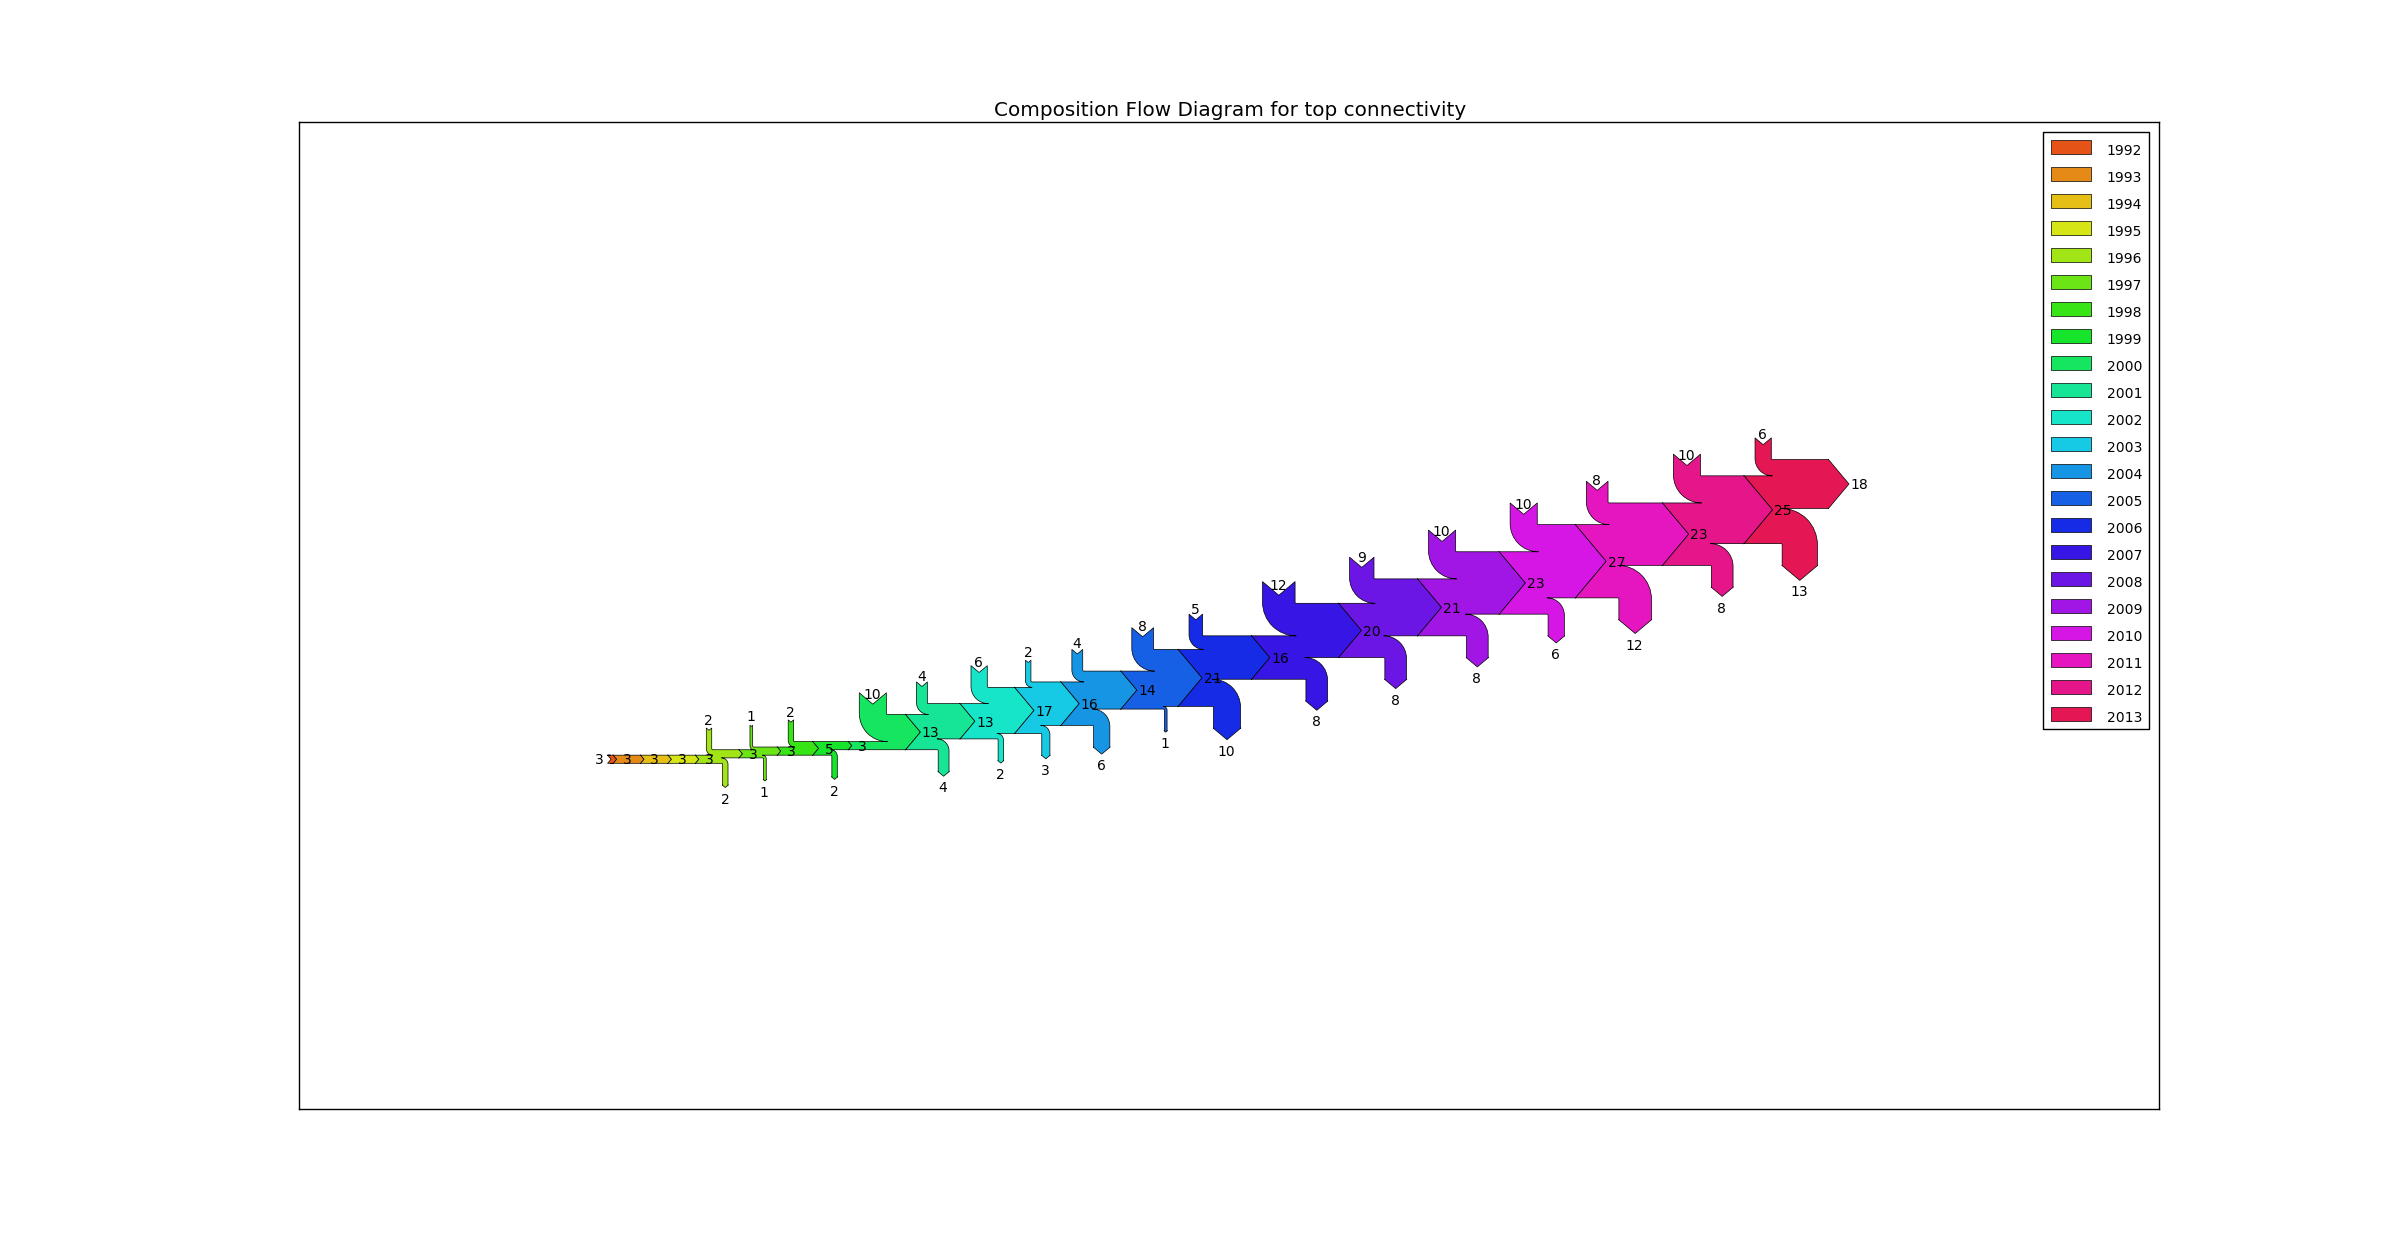
\includegraphics[scale=0.4]{figures/sankey_python}
\caption[Sankey diagram of the composition of each connectivity level.]{Evolution of the composition in the top connectivity level}
\label{fig:sankey}
\end{center}
\end{figure}
\end{landscape}


\subsection{Modeling robustness as median active live of individuals in the project}

In the network literature, robustness of networks is usually measured with simulations of failures (removing nodes at random) and attacks (removing nodes decrementally starting for the ones with higher degree) \citep{albert:2000}. However this is not a good way to model the evolution of participation in a FOSS project.

We use here the survival analysis approach \citep{miller:2011}, that according to our knowledge, is the first time that is applied to model the turn over in FOSS communities. In its origin, survival analysis, was focused on modeling lifespans of individuals and is still widely used in medicine. However, this kind of analysis can also be used to model any kind of duration. Thus we model the active life of a developer in the Python project to the period that this developer is contributing at least one line of source code. We consider a developer ``dead'' when she no longer contributes to the project.

To estimate the survival function from the empirical data we used the Kaplan-Meier estimator \citep{kaplan:1958} defined as:

$$
\hat{S}(t) = \prod_{t_i < t} \frac{n_i - d_i}{n_i}
$$

where $d_i$ are the number of ``death events'' at time $t$ and $n_i$ is the number of subjects at risk of death at time $t$. If we compute the Kaplan-Meier estimator for all developers (figure \ref{fig:survival_all}) we can see that the median time of a developer on the community, defined as the point in time where on average half of the population has abandoned the community, is 5 years. But if we consider separately the developers in the top level of the connectivity hierarchy (figure \ref{fig:survival_groups}), their median time is 10 years; but only 3 years for the developers that are not on the top of the connectivity hierarchy.

Although it is clear that the two survival functions depicted in figure \ref{fig:survival_groups} are different, we performed the log rank test, a common statistical test in survival analysis that compares two event series' generators. The test confirms that that the two series have different generator mechanisms and are significantly different.

Finally, given that we observe an important flow of new developers towards the top levels of the connectivity hierarchy; and also having established that the contributions of the developers in these top levels is significantly higher than other developers, it is interesting to analyze the personal trajectories of developers in the project. We model the active time of developers in the Python project using a Cox proportional hazards model with time-dependent covariates and right-censoring \citep[appendix on survival analysis]{fox:2002}.


\begin{figure}[H]
\centering
\subfloat[Survival Function for all developers]{
\label{fig:survival_all}
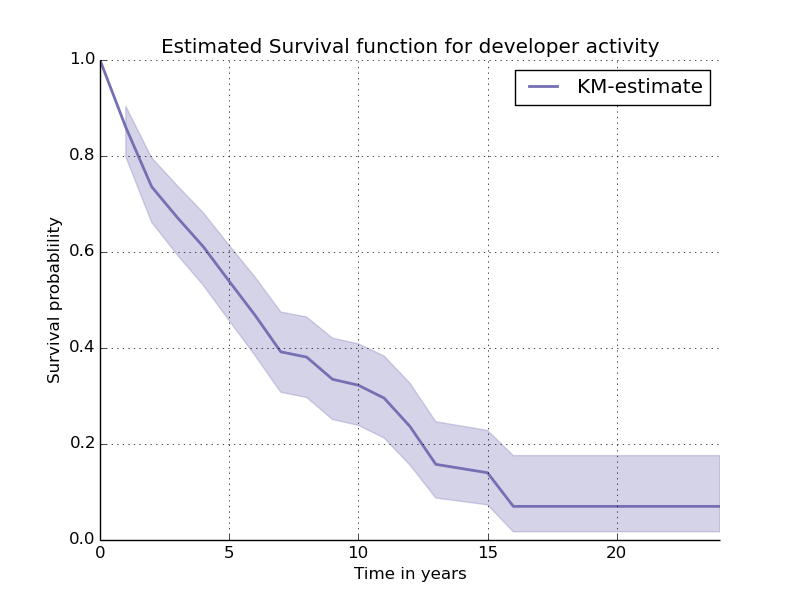
\includegraphics[scale=0.28]{figures/survival_all}
}
\hspace{.01in}
\subfloat[Survival Function for developers in the top connectivity level]{
\label{fig:survival_groups}
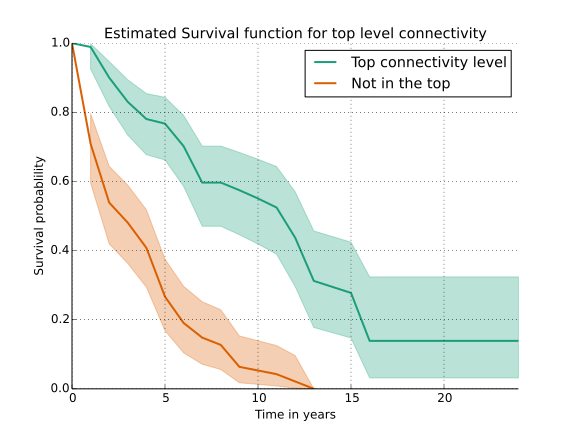
\includegraphics[scale=0.28]{figures/survival_top}
}
\label{fig:survival}
\caption[Survival function using the Kaplan-Meier estimate.]{Estimation of the survival function using the Kaplan-Meier estimate. The median time of a developer in the community, defined as the point in time where on average half of the population has abandoned the community, is 5 years if we consider all developers (left). But if we consider separately the developers in the top level of the connectivity hierarchy (right), their median time is 10 years; but only 3 years for the developers that are not on the top of the connectivity hierarchy.}
\end{figure}

We are interested in assessing the impact of being in the higher levels of the connectivity structure in terms of the expected active life of a developer in the project. The covariates in the model are: the number of accepted PEPs authored by each developer, the contributions of each developer to the Python project, measured as number of source code lines, the number of collaborators (ie second order neighbors in network terms) that each developer has in the cooperation network, the degree centrality and closeness of each developer in the cooperation network, the highest $k$ of a $k$-component in which the developer is embedded, and the \emph{Top connectivity level} dummy variable that equals to 1 if the developer is in the $k$-component of highest $k$ in the cooperation network for that time period, and 0 otherwise.


% Table created by stargazer v.5.2 by Marek Hlavac, Harvard University. E-mail: hlavac at fas.harvard.edu
% Date and time: dv, nov 18, 2016 - 12:37:21
% Requires LaTeX packages: dcolumn 
\begin{table}[!htbp] \centering 
  \caption{Survival Analysis: Cox proportional hazards regression model} 
  \label{python_cox_reg} 
\begin{tabular}{@{\extracolsep{5pt}}lD{.}{.}{-3} D{.}{.}{-3} D{.}{.}{-3} D{.}{.}{-3} } 
\\[-1.8ex]\hline 
\hline \\[-1.8ex] 
 & \multicolumn{4}{c}{\textit{Dependent variable:}} \\ 
\cline{2-5} 
\\[-1.8ex] & \multicolumn{4}{c}{Time active in the project} \\ 
\\[-1.8ex] & \multicolumn{1}{c}{(1)} & \multicolumn{1}{c}{(2)} & \multicolumn{1}{c}{(3)} & \multicolumn{1}{c}{(4)}\\ 
\hline \\[-1.8ex] 
 Total accepted PEPs & -0.118 & -0.105 & -0.113 & -0.103 \\ 
  & (0.111) & (0.114) & (0.118) & (0.118) \\ 
  Contributions & -0.00003 & -0.00002 & -0.00003 & -0.00002 \\ 
  & (0.00003) & (0.00003) & (0.00003) & (0.00003) \\ 
  Collaborators & -0.015 & 0.005 & -0.012 & 0.004 \\ 
  & (0.008) & (0.010) & (0.008) & (0.009) \\ 
  Degree Centrality & -50.770^{**} & -13.886 & -25.344 & -6.944 \\ 
  & (15.834) & (12.770) & (15.175) & (12.282) \\ 
  Closeness & 7.894 & 0.930 & 5.212 & 1.015 \\ 
  & (5.052) & (4.741) & (4.562) & (4.353) \\ 
  k-component number &  & -0.376^{***} &  & -0.295^{**} \\ 
  &  & (0.097) &  & (0.101) \\ 
  Top connectivity level &  &  & -1.885^{**} & -1.467^{*} \\ 
  &  &  & (0.617) & (0.657) \\ 
 \hline \\[-1.8ex] 
Observations & \multicolumn{1}{c}{754} & \multicolumn{1}{c}{754} & \multicolumn{1}{c}{754} & \multicolumn{1}{c}{754} \\ 
R$^{2}$ & \multicolumn{1}{c}{0.118} & \multicolumn{1}{c}{0.135} & \multicolumn{1}{c}{0.132} & \multicolumn{1}{c}{0.142} \\ 
Max. Possible R$^{2}$ & \multicolumn{1}{c}{0.396} & \multicolumn{1}{c}{0.396} & \multicolumn{1}{c}{0.396} & \multicolumn{1}{c}{0.396} \\ 
Log Likelihood & \multicolumn{1}{c}{-142.808} & \multicolumn{1}{c}{-135.379} & \multicolumn{1}{c}{-136.915} & \multicolumn{1}{c}{-132.501} \\ 
\hline 
\hline \\[-1.8ex] 
\textit{Note:}  & \multicolumn{4}{r}{$^{*}$p$<$0.05; $^{**}$p$<$0.01; $^{***}$p$<$0.001} \\ 
\end{tabular} 
\end{table} 


In order to fit the model, we divided the data in ``strata'' based on the value of ``tenure'' covariate which reflects the time a developer has been active in the project measured in years. Each stratum is permitted to have a different baseline hazard function, while the coefficients of the remaining covariates are assumed to be constant across strata. Stratification is most natural when a covariate takes on only a few distinct values, and when the effect of the stratifying variable is not of direct interest.

Finally the estimations of the variance and standard errors of the coefficients of the covariates of interest are robust, and clustered for each developer. This is necessary because in a proportional hazards model with time-dependent covariates, each individual has more than oner row in the database. Concretely, each individual has a row for each period of one year in which he or she has been an active contributor to the source code of the Python project. Tables \ref{desc_table_survival} and \ref{corr_table_survival} on appendix \ref{support-tables} show the descriptive statistics and the correlation matrix of the variables used in this model.

As we can see in table \ref{python_cox_reg}, the effect of being part of the top connectivity level is significant and negative with a coefficient of -1.467, meaning that it decreases the yearly hazard of leaving the project by a factor of $e^b = e^{-1.467} = 0.23$, that is, 77\%. This interpretation holds assuming that all other covariates remain constant. The coefficient for $k$-number ---the highest $k$ of a $k$-component in which the developer is embedded--- is also significative and negative with a coefficient of -0.295, which means that an increment of one connectivity level decreases the yearly hazard of leaving the project by a factor of $e^b = e^{-0.295} = 0.74$, that is, 26\%.

It is relevant that both measures of cohesion are significative and negative when included in the same model, although the $k$-component number it's significative at $p < 0.01$ and being part of the top component at $p < 0.05$. When these two variables are included in the model none of the control variables is significative. We can conclude that not only being at the top connectivity level has a relevant impact on the active life of a developer in a project, but also smaller increments in cohesion of the groups in which a developer is embedded have a significant impact on their active life in the project.

\section{Conclusion}

In this chapter we explored the dynamical dimension of the hierarchies that emerge on cooperation networks of FOSS projects. We defined cooperation networks as the patterns of relations among developers established while contributing to the project. The dynamic analysis, in this case, is not a longitudinal account of the changes in the hierarchy through time, but the analysis of the pace of renewal of individuals in the positions defined by the hierarchy. We propose that organizations ---and not only FOSS projects--- can be classified in a continuum depending on the pace of renewal of the individuals that occupy key positions in the hierarchy.

We showed that the structural cohesion model \citep{white:2001, moody:2003} is a solid theoretical framework to define cohesive groups ---$k$-components--- in collaboration networks. The nested structure of $k$-components nicely captures the hierarchy in the patterns of relations that individual contributors establish when working in a FOSS project. This hierarchy, on the one hand, reflects the empirically well established fact that in FOSS projects only a small fraction of the developers account for most of the contributions. And, on the other hand, refutes the naive views of early academic accounts that characterized FOSS projects as a flat hierarchy of peers in which every individual does more or less the same.

We also showed that the position of individual developers in the connectivity hierarchy of the collaboration network impacts significantly, on the one hand, on the volume of contributions that an individual does to the project. And, on the other hand, on the median life time of developers in the project. We argue that the latter is a better way to analyze robustness of FOSS projects than the classical random and targeted attacks that has been used to asses robustness in other kinds of networks.

Our main conclusion is that the connectivity structure of FOSS cooperation networks can be characterized as a dynamic hierarchy, where the top levels of this hierarchy are filled with new individuals at a high pace. This feature is key for understanding the mechanisms and dynamics that make FOSS communities able to develop long term projects, with high individual turnover, and yet achieve high impact and coherent results. Therefore, we can conclude that cooperation in FOSS communities has a structural dimension because membership in cohesive groups that emerge from the cooperation networks ---the repeated patterns of relations that the direct producers establish in the production process--- has an important and statistically significative impact on both the volume of individual contributions, and on the median active life of developers in a FOSS project.
